\documentclass[svgnames,dvipsnames,hyperref={bookmarks=false},usepdftitle=false]{beamer}
\usetheme{fby}

\title{The State of the Meta}
\author{Eugene Burmako (\href{https://twitter.com/xeno_by}{@xeno{\textunderscore}by})}
\institute{\'Ecole Polytechnique F\'ed\'erale de Lausanne \\ \texttt{http://scalameta.org/}}
\date{22 November 2014}
\hypersetup{pdfauthor={Eugene Burmako},pdftitle={The State of the Meta (in Scala)}}

\begin{document}

\titleframe

\begin{frame}{Outline}
\begin{itemize}
\item Why metaprogramming matters
\item The present (scala.reflect)
\item The future (scala.meta)
\end{itemize}
\end{frame}

\sectionframe{Why metaprogramming matters}

\begin{frame}{Metaprogramming is...}
\begin{quote}
Metaprogramming is the writing of computer programs that write or manipulate other programs or themselves as their data.
\end{quote}
\begin{flushright}
\textemdash Wikipedia
\end{flushright}
\end{frame}

\begin{frame}{Use case \#1: Code generation}

Sometimes you have to reach for a sledgehammer:

\begin{itemize}
\item High performance
\item Integration with external systems
\item Abstraction over heterogeneous datatypes
\end{itemize}

\end{frame}

\begin{frame}{Use case \#2: Advanced static checks}

Types are useful, but every now and then they fall short:

\begin{itemize}
\item Restrict the types of variables that are captured in closures
\item Ensure that communication between actors is sound
\item Prevent overflows or underflows in computation-heavy code
\end{itemize}

\end{frame}

\begin{frame}{Use case \#3: Advanced domain-specific languages}

Even flexible syntax and powerful types have their limits:

\begin{itemize}
\item LINQ
\item async/await
\item External DSLs
\end{itemize}

\end{frame}

\begin{frame}{Use case \#4: Tooling}

\begin{itemize}
\item Style checking
\item Refactoring
\item Incremental compilation
\item And much-much more
\end{itemize}

\end{frame}

\sectionframe{The present (scala.reflect)}

\begin{frame}{The present (scala.reflect)}

\begin{itemize}
\item Decent support for compile-time metaprogramming (macros)
\item Some support for runtime metaprogramming (reflection, codegen)
\item Hardcore compiler internals or reinvented wheels for everything else
\end{itemize}

\end{frame}

\begin{frame}[fragile]{Macros by example}

\begin{semiverbatim}
def createArray[T: ClassTag](size: Int, el: T) = \{
  val a = new Array[T](size)
  for (i <- 0 until size) a(i) = el
  a
\}

\end{semiverbatim}

\begin{itemize}
\item We want to write beautiful generic code, and Scala makes that easy
\item Unfortunately, abstractions oftentimes bring overhead
\end{itemize}
\end{frame}

\begin{frame}[fragile]{Macros by example}

\begin{semiverbatim}
Object createArray(int size, Object el, ClassTag tag) \{
  Object a = tag.newArray(size);
  for (int i=0; i<size; i++) ScalaRunTime.array_update(...);
  return a;
\}

\end{semiverbatim}

\begin{itemize}
\item Scala runs on the JVM, so polymorphic signatures have to be erased
\item Erasure leads to boxing and boxing creates significant slowdowns
\item The snippet above shows a sketch of what \texttt{createArray} compiles to
\end{itemize}
\end{frame}

\begin{frame}[fragile]{Macros by example}

\begin{semiverbatim}
def createArray[@specialized T: ClassTag](...) = \{
  val a = new Array[T](size)
  for (i <- 0 until size) a(i) = el
  a
\}

\end{semiverbatim}

\begin{itemize}
\item Methods can be specialized, but it's viral and heavyweight
\item Viral = the entire call chain needs to be specialized
\item Heavyweight = specialization leads to duplication of bytecode
\end{itemize}
\end{frame}

\begin{frame}[fragile]{Macros by example}

\begin{semiverbatim}
def createArray[T: ClassTag](size: Int, el: T) = \{
  val a = new Array[T](size)
  def specBody[@specialized T](a: Array[T], el: T) = \{
    for (i <- 0 until size) a(i) = el
  \}
  classTag[T] match \{
    case ClassTag.Int => specBody(
      a.asInstanceOf[Array[Int]], el.asInstanceOf[Int])
    ...
  \}
  a
\}
\end{semiverbatim}

\begin{itemize}
\item We want to specialize just as much as we need
\item But that's tiresome to do by hand, and this is where macros shine
\end{itemize}
\end{frame}

\begin{frame}[fragile]{Macros by example}

\begin{semiverbatim}
\alert{def specialized[T](x: => Any) = macro impl[T]}

def createArray[T: ClassTag](size: Int, el: T) = \{
  val a = new Array[T](size)
  \alert{specialized[T] \{}
    for (i <- 0 until size) a(i) = el
  \alert{\}}
  a
\}

\end{semiverbatim}

\begin{itemize}
\item \texttt{specialized} macro gets pretty code and transforms it into fast code
\item The transformation is carried out by an associated metaprogram \texttt{impl}
\item For more details, see \text{\color{blue}\href{http://lampwww.epfl.ch/\~hmiller/scala2013/resources/pdfs/paper10.pdf}{Bridging Islands of Specialized Code}}
\end{itemize}
\end{frame}

\begin{frame}{How macros work}

\begin{itemize}
\item We publish the language model as part of the standard distribution
\item \texttt{scala-reflect.jar} contains definitions of trees, symbols, types, etc
\item Macros are written against data structures from scala.reflect
\item And executed inside \texttt{scalac} which implements the scala.reflect API
\end{itemize}

\end{frame}

\begin{frame}[fragile]{How macros work}

\begin{semiverbatim}
def specialized[T](x: => Any) = macro impl[T]

def impl[T](\alert<1>{c: scala.reflect.macros.Context})
    \alert<2>{(x: c.Tree)(implicit T: c.WeakTypeTag[T])} = \{
  \alert<1>{import c.universe._}
  \alert<2>{val (specVars, specBody) = Helpers.specialize(x, T)}
  \alert<3>{q"""}
    \alert<3>{def specBody[@specialized T](..\$specVars) = \$specBody}
    \alert<3>{classTag[\$T] match \{ case ..\$cases \}}
  \alert<3>{"""}
\}
\end{semiverbatim}

\begin{itemize}
\only<1>{\item The entry point to compile-time metaprogramming is a context}
\only<1>{\item From there we can import a universe of trees, symbols, types, etc}
\only<2>{\item Reflection artifacts that model Scala code are first-class}
\only<2>{\item We can pass them around to/from helpers, can create new ones}
\only<3>{\item Upon completion, a macro returns a tree representing new code}
\only<3>{\item This tree will replace the macro invocation at the call site}
\end{itemize}

\end{frame}

\begin{frame}{There's more}

\begin{itemize}
\item Type providers
\item Automatic generation of typeclass instances
\item Language virtualization
\item Deep integration with external DSLs
\item For details see our \text{\color{blue}\href{http://scalamacros.org/paperstalks/2014-02-04-WhatAreMacrosGoodFor.pdf}{``What Are Macros Good For?''}} talk
\end{itemize}

\end{frame}

\sectionframe{The future (scala.meta)}

\begin{frame}{The future (scala.meta)}

\begin{itemize}
\item This year we set out on a journey to create an ultimate metaprogramming API
\item Here we'll tell you about our design decisions and their impact
\end{itemize}

\end{frame}

\begin{frame}{scala.meta principles}

\begin{itemize}
\item Language model should be independent of language implementations
\item Interface for syntax trees should be based on hygienic quasiquotes
\item Binaries should provide access to their attributed abstract syntax trees
\end{itemize}

\end{frame}

\begin{frame}{Principle \#1: Independent language model}

\begin{itemize}
\item \texttt{scala.reflect} grew organically from scalac internals
\item That was a nice shortcut to get things going easily
\item But in the long run dependence on scalac makes everything harder
\end{itemize}

\end{frame}

\begin{frame}[c, fragile]{Principle \#1: Independent language model}
\begin{center}
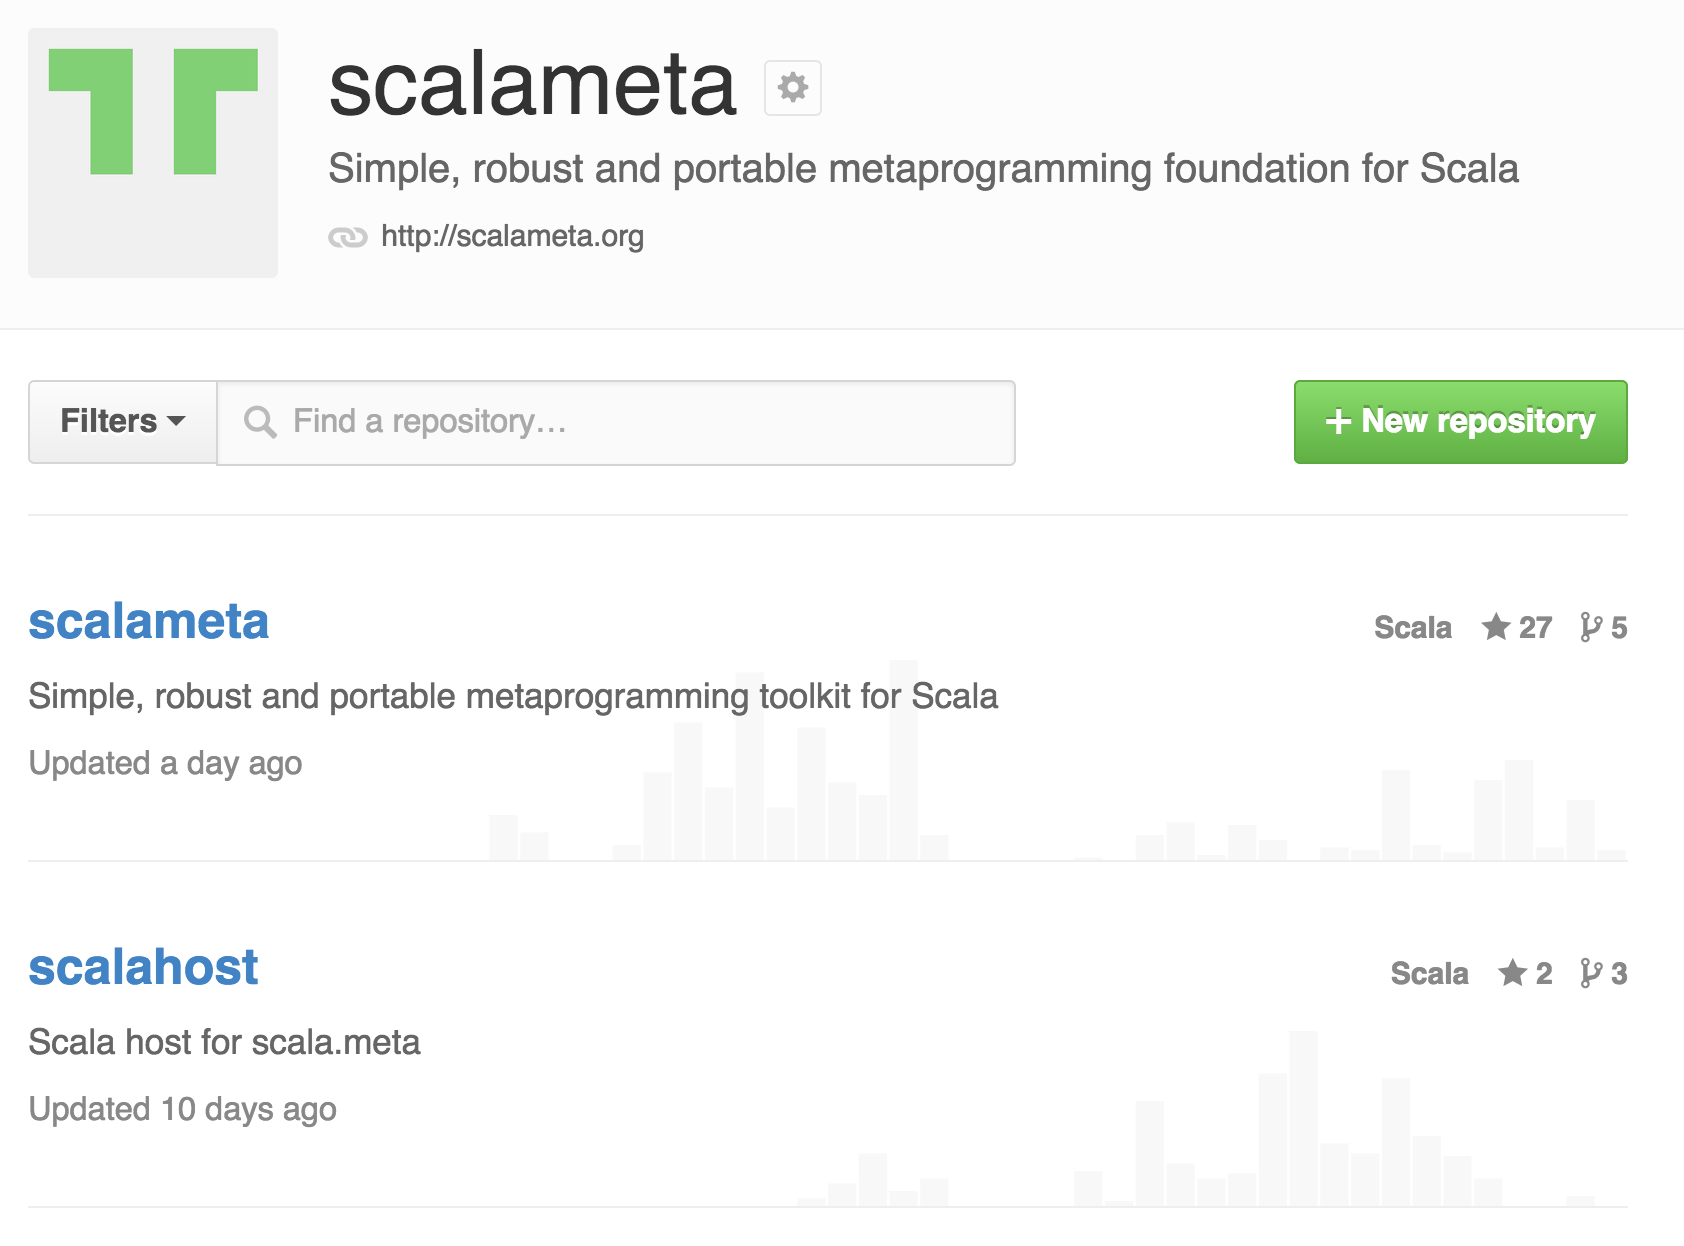
\includegraphics[height=7cm]{github.png}
\end{center}
\end{frame}

\begin{frame}{Principle \#1: Independent language model}

Diversity is real:
\begin{itemize}
\item ...Intellij (a reimplementation of Scala's typechecker)
\item ...Dotty (the next generation Scala compiler)
\item ...Typelevel (an experimental community fork)
\item ...Policy (a compiler/language technology fork)
\end{itemize}

\end{frame}

\begin{frame}[fragile]{Principle \#2: Hygienic quasiquotes}
\begin{semiverbatim}
ClassDef(
  NoMods,
  newTypeName("D"),
  Nil,
  Template(
    List(Ident(newTypeName("C"))),
    emptyValDef,
    List(DefDef(NoMods, nme.CONSTRUCTOR, ...))))

\end{semiverbatim}

\begin{itemize}
\item Once, the most reliable way to do ASTs was via vanilla datatypes
\item Above you can see what it took to say \texttt{class D extends C}
\item Needless to say, only brave souls cared to use such an API
\end{itemize}
\end{frame}

\begin{frame}[fragile]{Principle \#2: Hygienic quasiquotes}
\begin{semiverbatim}
val tree = q"class D extends C"
val q"class \$_ extends ..\$parents" = tree

\end{semiverbatim}

\begin{itemize}
\item Then we introduced quasiquotes, a template-based approach to ASTs
\item Quasiquotes became the highlight of the Scala 2.11 release
\item At this point our metaprogramming API started to look friendly
\end{itemize}
\end{frame}

\begin{frame}[fragile]{Principle \#2: Hygienic quasiquotes}
\begin{semiverbatim}
import foo.bar.C
val tree = q"class D extends C"
q"class C; \$tree"

\end{semiverbatim}

\begin{itemize}
\item The final puzzle to solve is prevention of name clashes
\item This is what is called hygiene of a metaprogramming API
\item Probably the most common pitfall in Scala macros at the moment
\end{itemize}

\end{frame}

\begin{frame}{Principle \#3: Persistent syntax trees}

\begin{itemize}
\item Every compilation produces attributed syntax trees
\item These trees contain a wealth of semantic information about programs
\item These trees get thrown away every time
\end{itemize}

\end{frame}

\begin{frame}{Principle \#3: Persistent syntax trees}

What if we saved attributed trees instead of throwing them away?
\begin{itemize}
\item Easy interpretation
\item Easy code analysis
\item And other neat metaprogramming tricks
\end{itemize}

\end{frame}

\begin{frame}[c, fragile]{Principle \#3: Persistent syntax trees}
\begin{center}
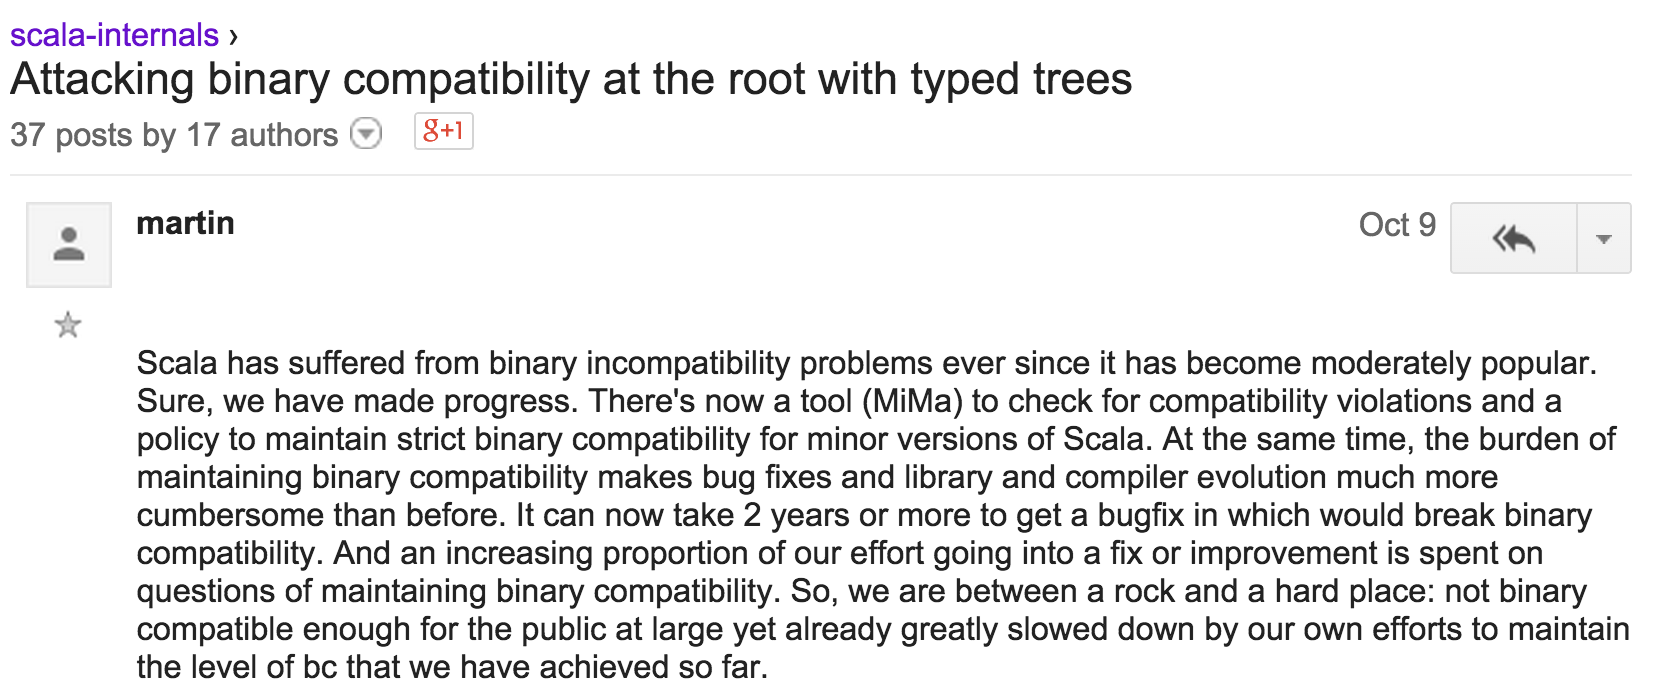
\includegraphics[height=5cm]{martin.png}
\end{center}
\end{frame}

\begin{frame}{Principle \#3: Persistent syntax trees}

It turns out that tree persistence is so much more:
\begin{itemize}
\item Separate the frontend and the backend of the compiler
\item Typed syntax trees become the new bytecode
\item Linker produces binaries native to target platforms
\item Solves bincompat problems and enables amazing optimizations!
\end{itemize}

\end{frame}

\begin{frame}{Our status}
\begin{itemize}
\item We have an initial design of the metaprogramming API
\item And are currently validating it on a number of use cases
\item Something publicly usable should appear next year
\item Most likely as a compiler plugin for Scala 2.11
\end{itemize}
\end{frame}

\sectionframe{Summary}

\begin{frame}{Summary}

\begin{itemize}
\item Metaprogramming is useful, and Scala programmers use it
\item You don't just grow a metaprogramming API from compiler internals
\item High tech is paramount for usability (quasiquotes, hygiene, etc)
\item Tree persistence can enable unexpected technological advances
\end{itemize}

\end{frame}

\end{document}